\documentclass{beamer}


\usepackage{amsmath}
\usepackage[style=alphabetic,url=true]{biblatex}
\usepackage{environ}
\usepackage{geometry}
\usepackage{graphicx}
\usepackage{tikz}
\usepackage[T2A]{fontenc}
\usepackage[utf8]{inputenc}
\usepackage[cache=false]{minted}
\usepackage{amsmath}
\usepackage{amsfonts}
\usepackage{amssymb}
\usepackage{calrsfs}
\usepackage{animate}
\usepackage{xmpmulti}


% \usetheme{Bergen}

\usecolortheme{beaver}

\setbeamertemplate{itemize item}[circle]
\setbeamertemplate{itemize subitem}{--}
\addtobeamertemplate{navigation symbols}{}{
  \usebeamerfont{footline}%
  \usebeamercolor[fg]{footline}%
  \hspace{1em}%
  \insertframenumber/\inserttotalframenumber
}
\graphicspath{ {./graphics/} }
\setminted[Python]{
  fontsize=\tiny
}
\BeforeBeginEnvironment{minted}{\medskip}
\AfterEndEnvironment{minted}{\medskip}
\usetikzlibrary{matrix}
\tikzset{
  stack/.style={
    matrix of nodes,
    nodes={
      fill=lightgray,draw,text=black,font=\sffamily\bfseries,
      text height=11pt,text depth=3pt,baseline=center, minimum width=1cm
    },
    column sep=-\pgflinewidth/2
  }
}

\title{
  Bitcoin and Cryptocurrency Technologies \\
  Lecture 7: Bitcoin Protocol
}

\author{Yuri Zhykin}
\date{Mar 20, 2025}

\begin{document}

\frame{\titlepage}

\begin{frame}
  \frametitle{Bitcoin Protocol}
  \begin{itemize}
  \item \textbf{Bitcoin Protocol} is a distributed protocol for producing a
    \textbf{limited amount} of \textbf{digital tokens (currency)},
    \textbf{provably assigning ownership} of the tokens to certain entities,
    giving those entities the ability to \textbf{irreversibly transfer (spend)}
    the ownership of the tokens to other entities and \textbf{preventing double
      transfer}.
  \item Previous attempts at digital currencies were unable to resolve the
    problem of \textbf{double spending} without central authority.
  \end{itemize}
\end{frame}

\begin{frame}
  \frametitle{Bitcoin Network Roles 1/2}
  \begin{itemize}
  \item Members of the Bitcoin Network are divided into the following classes:
    \begin{itemize}
    \item \textbf{full nodes} (validating nodes) - members that run Bitcoin Node
      software, propagating and validating blocks and transactions; these
      guarantee the \textit{strength-in-numbers} policy of the distributed
      Bitcoin protocol;
    \item \textbf{miners} (full nodes with mining hardware) - members that
      compute blocks and provide the \textit{computational security} of the
      network;
    \item \textbf{light nodes} - nodes that are only interested in particular
      parts of Bitcoin protocol, e.g. transactions and their corresponding
      blocks (Simplified Payment Verification nodes, mobile wallet software).
    \end{itemize}
  \end{itemize}
\end{frame}

\begin{frame}
  \frametitle{Bitcoin Network Roles 2/2}
  \begin{itemize}
  \item \textbf{Full nodes} ensure that miners do not mine invalid blocks
    (i.e. low chainwork blocks or blocks with invalid transactions);
  \item \textbf{Miners}
    \begin{itemize}
    \item cannot mine invalid blocks because these will immediately be rejected
      by the full nodes, which results in immediate loss of all resources spent
      on computing PoW,
    \item heavily invested in hardware and their only income is block rewards,
      so if the network is compromised, their investment loses value;
    \end{itemize}
  \item \textbf{Light nodes} only keep a chain of block headers (68 MiB of data
    as of March 2025) and validate only specific transactions.
  \end{itemize}
\end{frame}

\begin{frame}
  \frametitle{Limited Supply 1/4}
  \begin{itemize}
  \item Bitcoin Protocol incentivises miners to spend resources on PoW
    computation by allowing them to generate new bitcoin in the
    \textbf{coinbase} transactions.
  \item Additionally, miner claims fee of all transactions that were included in
    the block.
  \item Bitcoin is designed to have a \textbf{strictly limited supply} of the
    bitcoin tokens, so the amount of bitcoin generated in each new block is
    reduced over time.
  \item As block reward becomes smaller, miners rely more on transaction fees.
  \end{itemize}
\end{frame}

\begin{frame}
  \frametitle{Limited Supply 2/4}
  \begin{itemize}
  \item Every 210,000 blocks the reward is halved:
    \begin{itemize}
    \item 50 BTC (5,000,000,000 satoshis) in 2009-2012,
    \item 25 BTC (2,500,000,000 satoshis) in 2012-2016,
    \item 12.5 BTC (1,250,000,000 satoshis) in 2016-2020,
    \item 6.25 BTC (625,000,000 satoshis) in 2020-2024.
    \item 3.125 BTC (312,500,000 satoshis) since 2024.
    \end{itemize}
  \item Bitcoin block reward follows a geometric progression
    $$a_n = ar^n \text{, } a = 50 \text{, } r = \frac{1}{2}$$
    the sum of which is the total amount of bitcoin to ever exist:
    $$210000 \times \sum_{n = 1}^{n: a_n \geq 1} a_n = 210000 \times \frac{a(1 -
      r^n)}{1 - r} = 21000000$$
  \end{itemize}
\end{frame}

\begin{frame}
  \frametitle{Limited Supply 3/4}
  \begin{itemize}
  \item Bitcoins can be accidentally ``lost'' (the owner loses access to the key
    needed to unlock the lock script).
  \item Bitcoin can also be intentionally ``destroyed'' by sending coins to an
    address with an unknown key, for example
    \begin{small}
      $$1BitcoinEaterAddressDontSendf59kuE$$
    \end{small}
  \item According to some studies, around 600,000-1,100,000 bitcoins may belong
    to Satoshi Nakamoto from the early network period.
  \end{itemize}
\end{frame}

\begin{frame}
  \frametitle{Limited Supply 4/4}
  \begin{itemize}
  \item \href{https://bitcoinisdata.com}{bitcoinisdata.com}: 4-6 million
    bitcoins are likely lost forever
  \end{itemize}
  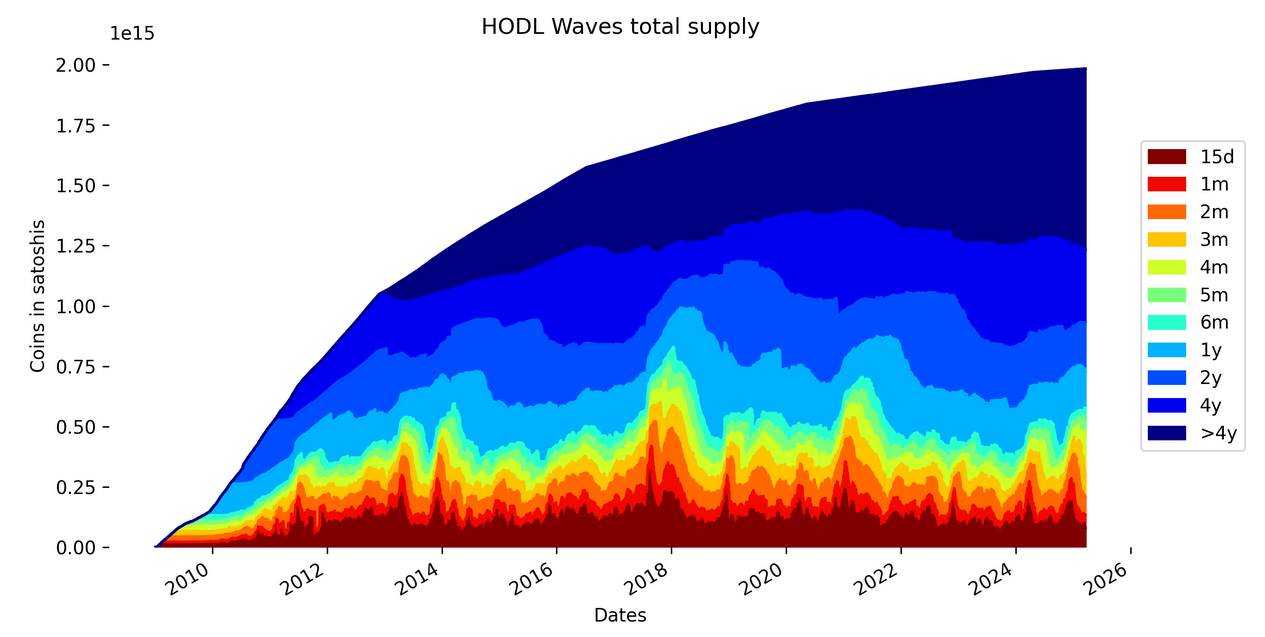
\includegraphics[width=\textwidth]{utxo-age}
\end{frame}

\begin{frame}
  \frametitle{Forks 1/2}
  \begin{itemize}
  \item \textbf{Soft fork} is a Bitcoin Protocol change that \textbf{restricts}
    the set of rules applied to blocks and transactions.
  \item \textbf{Some} of the blocks or transactions considered \textbf{valid} by
    the \textbf{old (non-upgraded) nodes} are considered \textbf{invalid} by the
    \textbf{new (upgraded) nodes}.
  \item Soft fork does not drop any nodes from consensus, but requires majority
    of the nodes to upgrade for the new rule to be enforced.
  \item Old nodes can still ``play by the old rules''.
  \end{itemize}
\end{frame}

\begin{frame}
  \frametitle{Forks 2/2}
  \begin{itemize}
  \item \textbf{Hard fork} is a Bitcoin Protocol change that \textbf{relaxes}
    the set of rules applied to blocks and transactions:
  \item \textbf{Some} of the blocks or transactions considered \textbf{valid} by
    the \textbf{new (upgraded) nodes} are considered \textbf{invalid} by the
    \textbf{old (non-upgraded) nodes}.
  \item Hard fork effectively drops old nodes from consensus, so it requires all
    nodes to upgrade to avoid the network split.
  \item Nodes that ``play by the old rules'' are separated from the main network
    into a separate network.
  \end{itemize}
\end{frame}

\begin{frame}
  \frametitle{Network Hashrate 1/2}
  \begin{itemize}
  \item For \textbf{hash-based Proof-of-Work systems}, the computing power can
    be conveniently measured by \textbf{hashrate} - \textbf{hashes computed per
      second} (H/s).
  \item Current total \textbf{hashrate} of the Bitcoin network is approximately
    804 Eh/s ($804 \times 10^{18} = $ 804,000,000,000,000,000 H/s), compared to
    375 Eh/s in 2022.
  \item As block rewards attract more miners, the total computing power of
    Bitcoin network increases.
  \end{itemize}
\end{frame}

\begin{frame}
  \frametitle{Network Hashrate 2/2}
  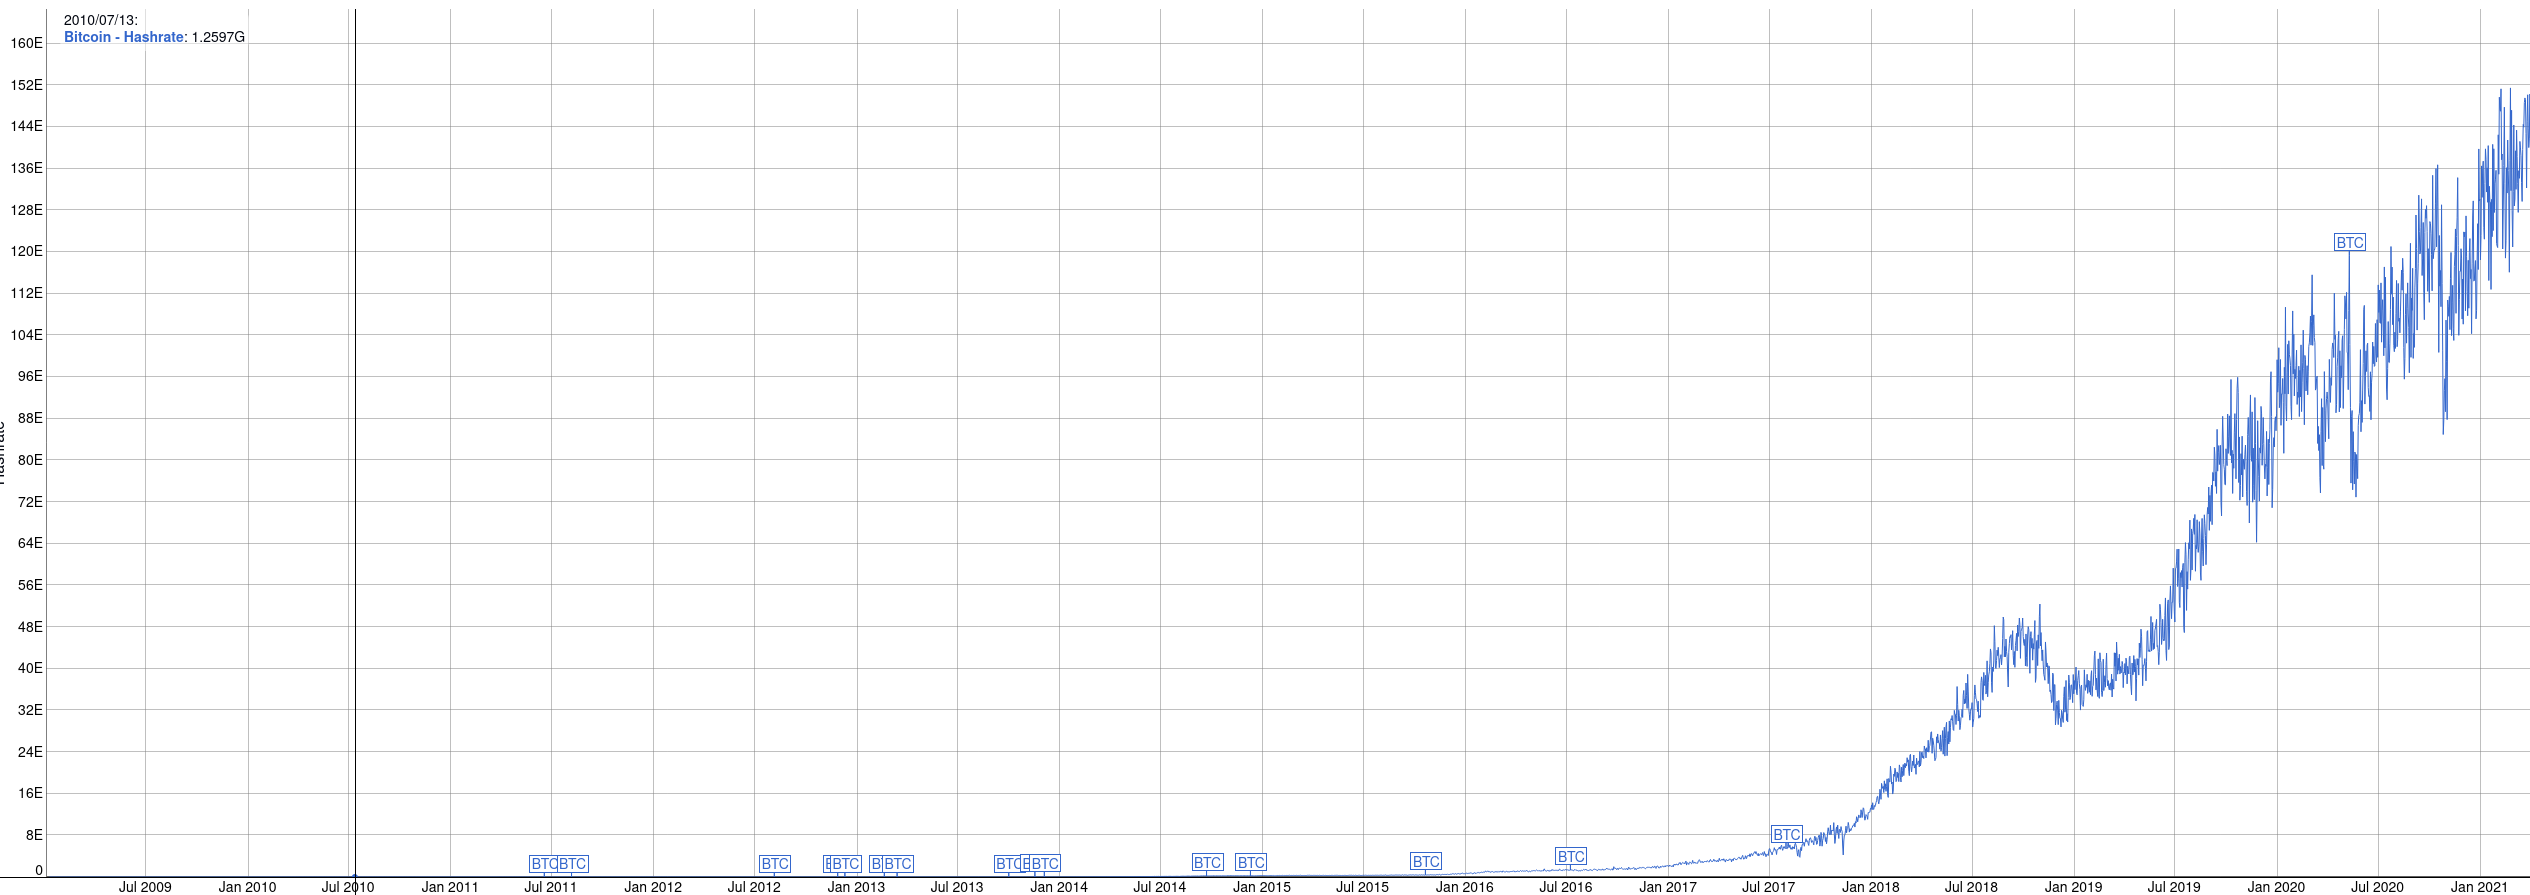
\includegraphics[width=\textwidth]{hashrate}
\end{frame}

\begin{frame}
  \frametitle{Difficulty Adjustment}
  \begin{itemize}
  \item In order to accomodate to the increasing computing power of the network,
    Bitcoin Protocol includes the \textbf{difficulty adjustment process}.
  \item Every 2,016 blocks (approximately 2 weeks), the difficulty of the PoW
    task is recalculated based on the last 2,016 blocks:
    \begin{itemize}
    \item if the averate time between last 2,016 blocks is \textit{more than 600
        seconds}, the \textit{difficulty is decreased} (the \textit{PoW target
        is increased}), otherwise the \textit{difficulty is increased} (the
      \textit{PoW target is decreased}).
    \end{itemize}
  \item The PoW difficulty is represented as the \textbf{PoW target} 256-bit
    number, which is in turn encoded as \textbf{bits} value and included in the
    block header, so the PoW solution can be verified independently.
  \end{itemize}
\end{frame}

\begin{frame}
  \frametitle{The End}
  \begin{center}
    Thank you!
  \end{center}
\end{frame}

\end{document}

%%% Local Variables:
%%% mode: latex
%%% TeX-master: t
%%% End:
